\documentclass[10pt,a4paper]{report}
\usepackage[latin1]{inputenc}
\usepackage{amsmath}
\usepackage{amsfonts}
\usepackage{amssymb}
\usepackage{graphicx}
\usepackage{listings}
\usepackage{color}
\usepackage[width=17.00cm, height=25.00cm]{geometry}
\renewcommand\thesection{\noindent{}}
\definecolor{codegreen}{rgb}{0,0.6,0}
\definecolor{codegray}{rgb}{0.5,0.5,0.5}
\definecolor{codepurple}{rgb}{0.58,0,0.82}
\definecolor{backcolour}{rgb}{0.95,0.95,0.92}

\lstdefinestyle{mystyle}{
	backgroundcolor=\color{backcolour},   
	commentstyle=\color{codegreen},
	keywordstyle=\color{magenta},
	numberstyle=\tiny\color{codegray},
	stringstyle=\color{codepurple},
	basicstyle=\footnotesize,
	breakatwhitespace=false,         
	breaklines=true,                 
	captionpos=b,                    
	keepspaces=true,                 
	numbers=left,                    
	numbersep=5pt,                  
	showspaces=false,                
	showstringspaces=false,
	showtabs=false,                  
	tabsize=2
}
\lstset{style=mystyle}
\begin{document}
	\section{Implementazione algoritmo PC}
	A lezione abbiamo visto che dato un insieme di $n$ variabili casuali:
	$$
	\{X_1,X_2,\dots,X_n\}
	$$
	� possibile definire su di esso la matrice varianza covarianza come segue:
	$$
	\Sigma \in \mathbb{R}^{n\times n} = \begin{bmatrix}
	E[(X_1-\overline{X_1})(X_1-\overline{X_1})] & E[(X_1-\overline{X_1})(X_2-\overline{X_2})] & \dots & E[(X_1-\overline{X_1})(X_n -\overline{X_n})]  \\ 
	E[(X_2-\overline{X_2})(X_1-\overline{X_1})] & E[(X_2-\overline{X_2})(X_2-\overline{X_2})] & \dots & E[(X_2-\overline{X_2})(X_n -\overline{X_n})]  \\ 
	. & . & . & . \\
	. & . & . & . \\
	. & . & . & . \\
	. & . & . & . \\
	E[(X_n-\overline{X_n})(X_1-\overline{X_1})] & E[(X_n-\overline{X_n})(X_2-\overline{X_2})] & \dots & E[(X_n-\overline{X_n})(X_n -\overline{X_n})]  \\ \end{bmatrix} 
	$$
	Questa matrice � simmetrica definita positiva, dunque da un punto di vista puramente matematico � \emph{sempre} non singolare, quindi \emph{sempre} invertibile.\\
	La sua inversa $\Sigma^{-1}$ \normalsize � chiamata matrice di precisione, ed � legata alla \emph{correlazione parziale} tra le $n$ variabili casuali secondo la relazione:\\
	$$
	\rho_{ij}.rest = \frac{-\sigma^{ij}}{\sqrt{\sigma^{ii}\sigma^{ij}}}\;\;(1.0)
	$$
	Dove:
	$\rho_{ij}.rest$ � il coefficiente di correlzione parziale fra la variabile $X_i$ e la variabile $X_j$ condizionato a tutte le rimanenti, e $\sigma^{ij}$ � l'$i,j-esimo$ elemento di $ \Sigma^{-1}$.\\
	Vale inoltre la seguente relazione:
	$$
	X_i \perp\mkern-10mu\perp X_j\;|\;rest \Leftrightarrow \rho_{ij}.rest = 0
	$$
	Il  PC algorithm costruisce lo scheletro del DAG con la seguente logica "grossolana":
	\begin{itemize}
		\item Inizializza il grafo come isomorfo a $K_{n\times n}$
		\item Per ogni coppia ordinata $(i,j)$ di nodi (variabili) tale per cui esiste un arco non direzionato da $i$ a $j$:
		\begin{itemize}
			\item controlla se una certa disequazione di test � soddisfatta
			\item se si, allora le due variabili sono indipendenti dato il resto, quindi l'arco fra i due rispettivi nodi nel grafo non deve esistere
		\end{itemize}
	\end{itemize}
	La disequazione che ho chiamato "di test" utilizza la trasformata $z$ di Fisher sulla matrice delle correlazioni parziali (che pu� essere ottenuta da $\Sigma^{-1}$), ed � la seguente:
	$$
	\sqrt{N-|{K}|-3}\;|{z(i,j|rest)}| \le \Phi^{-1}(1-\frac{\alpha}{2})
	$$
	Dove
	$N$ � il numero di variabili, $|K|=l=$ numero di vicini del nodo $i$, escluso il nodo $j$, $z$ � la trasformata di Fisher, $\Phi^{-1}(1-\frac{\alpha}{2})$ � l'inversa della funzione $\Phi$ distribuzione cumulativa della Normale, valutata in $(1-\frac{\alpha}{2})$ e infine $\alpha$ � detto \emph{tuning parameter}.\\*
	
	Per provare a valutare le performance di questo algoritmo, ho implementato il seguente codice python:
\begin{lstlisting}[language=Python]
def pc_algorithm(a,sigma_inverse):
	l = - 1
	n = len(sigma_inverse)
	z = lambda i,j : -sigma_inverse[i][j]/((sigma_inverse[i][i]*sigma_inverse[j][j])**0.5)
	act_g = complete(n)
	act = 0
	while l<n-1:
		l = l + 1
		for i in range(0,n):
			for j in range(i+1,n):
				if(act_g[i][j]!=1):	
					continue
				adjacents = adj(i,act_g)
				if len(adjacents)==0:
					continue
				act_set = setdiff(adjacents,[j])
				all_k = findsubsets(act_set, l)
				counter = 0
				while(act_g[i][j]!=0):
					if(counter >= len(all_k)):
						break
				K = all_k[counter];
				counter = counter+1
				if test(n,z,i,j,a,K):
					act_g[i][j] = 0
	for i in range(0,n):
		for j in range(0,n):
			if i>j:
				act_g[i][j] = act_g[j][i]
	return act_g;
	\end{lstlisting}
\section{Problemi}
Non sono ovviamente sicuro di aver implementato correttamente l'algoritmo in se, ma nello specifico un primo problema � stato quello di definire la trasformata $z$. Infatti la definisco come una funzione anonima che, data la matrice $\Sigma^{-1}$ mi restituisce la correlazione parziale di $i,j$ dato il resto, secondo la relazione $(1.0)$:
\begin{lstlisting}
z(i,j) = sigma_inverse[i][i]/sqrt(sigma_inverse[i][i]*sigma_inverse[j][j])
\end{lstlisting}
Non sono sicuro che questo sia corretto perch� il coefficiente di correlazione parziale andrebbe calcolato dato $K$, e non date tutte le altre variabili.\\
Un altro problema riguarda invece la funzione $\Phi^{-1}$, infatti non posso pensare di calcolarla direttamente in quanto non � esprimibile come combinazione lineare di funzioni analitiche e/o polinomiali, l'unica cosa che posso fare � approssimarla. Infatti:
$$
\Phi(x) = \frac{1}{\sqrt\pi} \int_0^x e^{-t^2} dt
$$
� un integrale irrisolvibile in forma chiusa ed esplicita.\\
Ho scelto di utilizzare la seguente approssimazione nota della funzione quantile $\Phi^{-1}$:
$$
\Phi^{-1}(p) = \sqrt2\;erf^{-1}(2p-1)
$$
Dove $erf^{-1}$ � a sua volta l'inversa della \emph{error function}, la quale necessita a sua volta di essere approssimata:
$$
erf^{-1}(x) = sgn(x)\sqrt{\sqrt{\left(\frac{2}{\pi a}+\frac{ln(1-x^2)}{2}\right)^2-\frac{ln(1-x^2)}{a}}-\left(\frac{2}{\pi a}+ \frac{ln(1-x^2)}{2}\right)}$$
Una buona approssimazione la si ottiene ponendo $a = 0.147$
\begin{lstlisting}[language=Python]
def test(n,z,i,j,a,K):
	root = (n-len(K)-3)**0.5
	return root*abs(z(i,j)) <= phi(1-a/2)

def phi(p):
	return (2**0.5)*erfinv(2*p-1)
	
def erfinv(x):
	sgn = 1
	a = 0.147
	PI = numpy.pi
	if x<0:
		sgn = -1
	temp = 2/(PI*a) + numpy.log(1-x**2)/2
	add_1 = temp**2
	add_2 = numpy.log(1-x**2)/a
	add_3 = temp
	rt1 = (add_1-add_2)**0.5
	rtarg = rt1 - add_3
	return sgn*(rtarg**0.5)
\end{lstlisting}
Un ultimo problema � che, generando dati casualmente, spesso ottengo anche matrici varianza-covarianza singolari in aritmetica finita, ma questo mi sembra che ce lo disse anche lei a lezione, quindi lo considero normale.

\section{Output}
La prima cosa che ho notato � che per $n>10$ variabili, i tempi di esecuzione sono molto lunghi.\\
Allego alcune immagini di grafi prodotti utilizzando il seguente dataset di 7 variabili generato in maniera casuale:
\tiny
$$
\begin{bmatrix}
0.1298712897211212 & 0.2112987219871212 & 0.1749521075950111 & 0.2156423156412200 & 0.0215615646515618 & 0.3231256154842521 & 0.1235484556489215 & \\
1.9741980022248782 & 0.8451937696200296 & 1.1799283254919182 & 0.6031724223406041 & -0.6566008384851423 & -1.0064929865840662 & 3.4676455398519845 & \\
3.100078139389854 & -0.7838869190170845 & 5.165622481002579 & 3.1184726581121383 & 4.899115147443788 & 1.870911939491902 & 1.5530716047378323 & \\
5.198030621914989 & 2.8160245411363602 & 5.482744040414655 & 2.17400869757652 & 8.353322676841408 & 2.4365539380996406 & 0.6299492890543488 & \\
4.1699869117111215 & 9.644663893776446 & 4.189526185481068 & -1.0367886406038753 & 5.959916183783191 & 5.331092113213319 & 3.9619019745126614 & \\
4.376395614608083 & 10.209356572618773 & -1.201476701612889 & -1.7526211220068442 & 1.2869284076136944 & 13.388500730751154 & 2.7765624095474357 & \\
-0.430623316687897 & 1.6433833402269427 & -10.033331689878722 & 8.137353672070207 & -2.3771004289730833 & -0.55908452236672 & 6.661604133285603 & \\

\end{bmatrix}
$$
\begin{figure}[h]
	\centering
	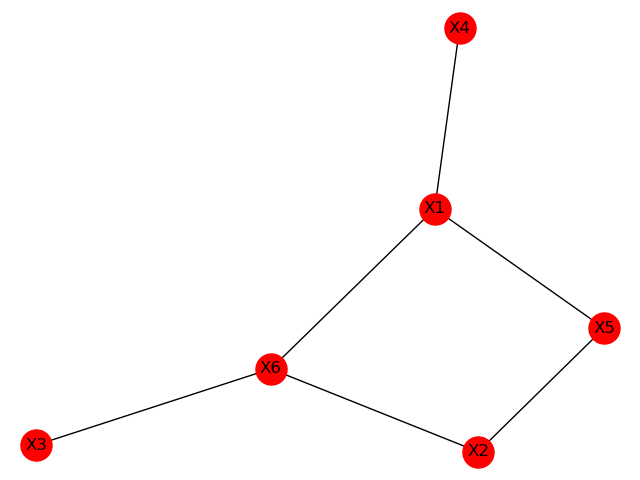
\includegraphics[scale=0.5]{Figure_1}
	\caption{Dataset casuale, alpha = 0.20}
	\label{fig:figure1}
\end{figure}
\begin{figure}[h]
	\centering
	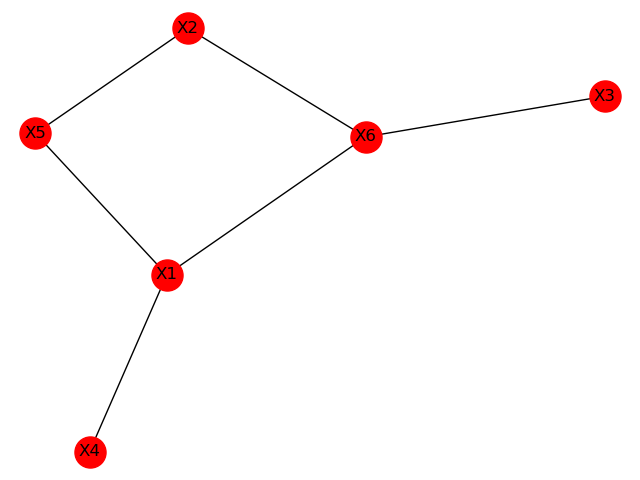
\includegraphics[scale=0.65]{Figure_2}
	\caption{Dataset casuale, alpha = 0.50}
	\label{fig:figure2}
\end{figure}
\normalsize
\newpage
Utilizzando invece direttamente la matrice $\Sigma^{-1}$ del butterfly model ottengo:\\*
\begin{figure}[h]
	\centering
	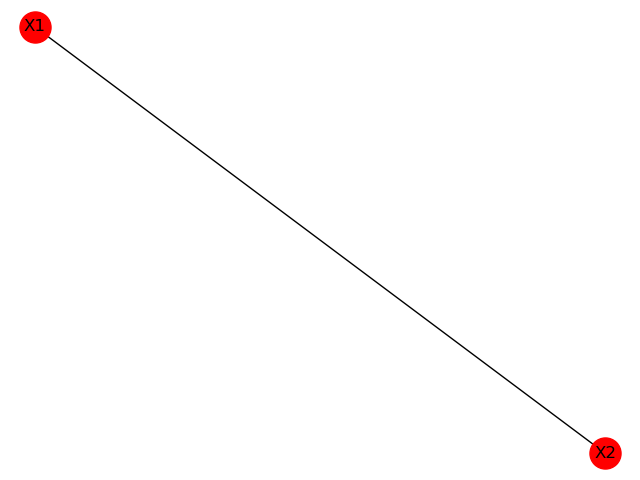
\includegraphics[scale=0.65]{Figure_3}
	\caption{Butterfly model, alpha = 0.95}
	\label{fig:figure3}
\end{figure}\\*
Il che � senza dubbio sbagliato, solo con alpha molto elevato ottengo un grafo non vuoto che comunque dovrebbe essere il modello a farfalla, ed � un segmento. Le volevo chiedere appunto una mano a capire dove fosse il, o pi� probabilmente gli, errori. Allego anche il codice completo.
\begin{lstlisting}[language=Python]
import itertools
import copy
import numpy
import graphtools

def matstr(A):
tos = ""
for row in A:
tos = tos + str(row)+"\n"
return tos

def complete(n):
A = list()
for i in range(0,n):
row = list()
for j in range(0,n):
if i == j:
row.append(0)
else:
row.append(1)
A.append(row)
return A

def setdiff(A,B):
ret_set = copy.copy(A)
for x in B:
if x in A:
ret_set.remove(x)
return ret_set

def adj(i,G):
adjacents = list()
for j in range(0,len(G[i])):
if i!=j and G[i][j] == 1:
adjacents.append(j)
return adjacents

def findsubsets(S,l):
return list(itertools.combinations(S,l))

def erfinv(x):
sgn = 1
a = 0.147
PI = numpy.pi
if x<0:
sgn = -1
temp = 2/(PI*a) + numpy.log(1-x**2)/2
add_1 = temp**2
add_2 = numpy.log(1-x**2)/a
add_3 = temp
rt1 = (add_1-add_2)**0.5
rtarg = rt1 - add_3
return sgn*(rtarg**0.5)

def phi(p):
return (2**0.5)*erfinv(2*p-1)

def test(n,z,i,j,a,K):
root = (n-len(K)-3)**0.5
# print str(root*abs(z(i,j)))+"<="+str(phi(1-a/2))+"?"
return root*abs(z(i,j)) <= phi(1-a/2)

def meanof(dataset):
n = len(dataset[0])
m = []
for i in range(0,n):
m.append(0.0)
datasize = len(dataset)
for i in range(0,datasize):
for j in range(0,n):
m[j] = m[j] + float(dataset[i][j])
for i in range(0,n):
m[i] = m[i] / datasize
return m

def zeros(n,m):
zer = []    
for i in range(0,n):
row = []
for j in range(0,m):
row.append(0)
zer.append(row)
return zer

def getcol(i,matrix):
col = []
for row in matrix:
col.append(row[i])
return col

def sigma(dataset,means):
n = len(means)
sigma = zeros(n,n)
for i in range(0,n):
for j in range(0,n):
dset_i = getcol(i,dataset)
dset_j = getcol(j,dataset)
means_i = means[i]
means_j = means[j]
sigma[i][j] = covar(dset_i,dset_j,means_i,means_j)
return sigma

def covar(X,Y,ux,uy):
n = len(X)
s = 0
for i in range(0,n):
s = s +(X[i] - ux)*(Y[i] - uy);
return float(s)/n

def getSigma(dataset):
means = meanof(dataset)
return sigma(dataset,means)

def getInverse(A):
return numpy.linalg.inv(A)

def pc_algorithm(a,sigma_inverse):
l = - 1
n = len(sigma_inverse)
z = lambda i,j : -sigma_inverse[i][j]/((sigma_inverse[i][i]*sigma_inverse[j][j])**0.5)
act_g = complete(n)
act = 0
while l<n-1:
l = l + 1
for i in range(0,n):
for j in range(i+1,n):
if(act_g[i][j]!=1):
continue
adjacents = adj(i,act_g)
if len(adjacents)==0:
continue
act_set = setdiff(adjacents,[j])
all_k = findsubsets(act_set, l)
counter = 0
while(act_g[i][j]!=0):
if(counter >= len(all_k)):
break
K = all_k[counter];
counter = counter+1
if test(n,z,i,j,a,K):
act_g[i][j] = 0
for i in range(0,n):
for j in range(0,n):
if i>j:
act_g[i][j] = act_g[j][i]
return act_g;

def rand_set(X,Var):
n = len(X)
rset = []
for i in range(0,n):
rset.append(numpy.random.normal(X[i],Var[i],n))
return rset; 

def make_graph_from_dataset(dataset,alpha):
sigma = getSigma(dataset)
sigma_inverse = getInverse(sigma)
return pc_algorithm(alpha,sigma_inverse)

def plot(adj_matrix,varnames):
graphtools.plot_graph(adj_matrix,varnames)

def get_rand_dataset(dim):
return rand_set(range(0,dim),range(0,dim))

def butterfly():
return [[0.8, 0.5, 0, 0.6],[0.5, 1.4, -0.6, 0.4],[0, -0.6, 1.2, -0.3],[0.6, 0.4, -0.3, 1]]

if __name__ == '__main__':
varnames = ['X1','X2','X3','X4']
alpha = 0.95
G = pc_algorithm(alpha,butterfly())
plot(G,varnames)
\end{lstlisting}
\end{document}